% !Mode:: "TeX:UTF-8"
% !TEX program  = xelatex
\documentclass[a4paper]{article}
\usepackage{amsmath}
\usepackage{amssymb}
\usepackage{ctex}
%\usepackage{braket}
%\usepackage[european]{circuitikz}
\usepackage{multirow}
\usepackage{float}
\usepackage{graphicx}
\usepackage{geometry}
\geometry{left=2.5cm,right=2.5cm,bottom=2.5cm,top=2.5cm}
\title{\Huge 近代物理实验报告\\\huge 实验1.1:NaI(Tl)闪烁谱仪系列实验---\\\LARGE 1.1.2:$\gamma$辐射的能量和强度测量}
\author{xy\quad 学号\quad 匡亚明学院}
\date{2019年2月29日}
\begin{document}
\maketitle
\bibliographystyle{unsrt}
%--------main-body------------

\section{引言}
闪烁探测器是利用某些物质在射线作用下受激发光的特性来探测射线的仪器。它们的主要优点是:既能探测各种带电粒子,又能探测中性粒子;既能测量粒子强度,又能测量粒子能量;且探测效率高,分辨时间短。它在核物理研究和放射性同位素测量中得到广泛的应用。本实验目的是了解NaI(Tl)闪烁谱仪的原理、特性与结构,掌握NaI(Tl)闪烁谱仪的使用方法和$\gamma$射线能谱的刻度,学会NaI(Tl)闪烁谱仪的应用。

\section{实验目的}
1. 了解NaI(Tl)闪烁谱仪的组成,基本特性及使用方法。
2. 掌握测量$\gamma$射线的能量和强度的基本方法。

\section{实验仪器}
NaI(Tl)闪烁谱仪。

\section{实验原理}

\subsection{射线与物质的相互作用}
射线与物质的相互作用主要是光电效应、康普顿散射和正、负电子对产生三种过程。
\begin{enumerate}
	\item 光电效应:入射$\gamma$粒子把能量全部转移给原子中的束缚电子,而把束缚电子打出来形成光电子。由于束缚电子的电离能$E_1$一般远小于入射$\gamma$射线能量$E_{\gamma}$ ,所以光电子的动能近似等于入射$\gamma$射线的能量。
	      \begin{equation*}
		      E_{\text{光电}} = E_{\gamma} - E_1 \approx E_{\gamma}
	      \end{equation*}
	      \begin{figure}[!h]
		      \centering
		      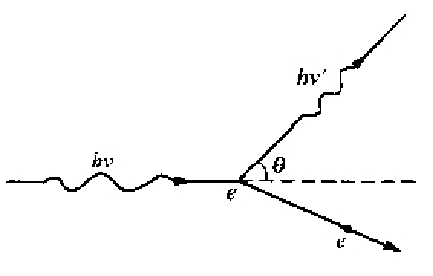
\includegraphics[width=0.4\textwidth]{fig/fig1.pdf}
		      \caption{康普顿散射示意图}\label{fig1}
	      \end{figure}

	\item 康普顿散射:核外电子与入射$\gamma$射线发生康普顿散射示意如图。设入射$\gamma$光子能量为$h\nu$,散射光子能量为$h\nu^{'}$,则反冲康普顿电子的动能$E_{\gamma}$
	      \begin{equation*}
		      E_{\gamma} = h\nu - h\nu^{'}
	      \end{equation*}
	      康普顿散射后散射光子能量与散射角$\theta$的关系为
	      \begin{eqnarray}
		      h\nu^{'} = \frac{h\nu}{1+\alpha(1-\cos\theta)}\label{eq1}\\
		      \alpha = \frac{h\nu}{m_ec^2}\notag
	      \end{eqnarray}
	      $\alpha$为入射$\gamma$射线能量与电子静止质量之比。由上式可得,当$\theta=0$时,$h\nu =h\nu^{'}$。这时$E_e=0$,即不发生散射;当$\theta=180^{\circ}$时,散射光子能量最小,它等于$\frac{h\nu}{1+2\alpha}$,这时康普顿电子的能量最大,为
	      \begin{equation}
		      E_{e(max)} = h\nu\cdot\frac{2\alpha}{1+2\alpha}\label{eq2}
	      \end{equation}
	      所以康普顿电子能量在0至$h\nu\cdot\frac{2\alpha}{1+2\alpha}$之间变化。
	\item 正、负电子对产生:当$\gamma$射线能量超过$2m_ec^2$(1.022MeV)时,$\gamma$光子受原子核或电子的库伦场的作用可能转化成正、负电子对。入射$\gamma$射线的能量越大,产生正、负电子对的几率也越大。在物质中正电子的寿命是很短的,当它在物质中消耗尽自己的动能,便同物质原子中的轨道电子发生湮没反应而变成一对能量各为0.511MeV的$\gamma$光子。
\end{enumerate}

\subsection{核衰变的统计规律}
在重复的放射性测量中,即使保持完全相同的实验条件(例如放射源的半衰期足够长,在实验时间内可以认为其活度基本上没有变化;源与探测器的相对位置始终保持不变;每次测量时间不变;测量仪器足够精确,不会产生其他的附加误差等),每次的测量结果并不完全相同,而是围绕着其平均值上下涨落,有时甚至有较大的差别。这种现象就叫做放射性计数的统计性。

放射性计数的这种统计性反映了放射性原子核衰变本身固有的特性,与使用的测量仪器及技术无关。放射性原子核衰变的统计分布可以根据数理统计分布的理论来推导。放射性原子核衰变的过程是一个相互独立彼此无关的过程,即每一个原子核的衰变是完全独立的,和别的原子核是否衰变没有关系,而且哪一个原子核先衰变,哪一个原子核后衰变也是纯属偶然的,并无一定的次序,因此放射性原子核的衰变可以看成是一种伯努里实验问题。设在$t=0$时,放射性原子核的总数是$N_0$,在$t$时间内将有一部分核发生了衰变。已知任何一个核在$t$时间内衰变的概率为$p = (1-e^{-\lambda t})$,不衰变的概率为$q = 1 - p = e^{-\lambda t}$。$\lambda$是该放射性原子核的衰变常数。利用二项式分布可以得到在$t$时间内有$n$个核发生衰变的概率$p(n)$为
\begin{equation}
	p(n) = \frac{N_0!}{(N_0 - n)!n!}(1-e^{-\lambda t})^n(e^{-\lambda t})^{N_0 - n}\label{eq3}
\end{equation}
在$t$时间内,衰变掉的粒子平均数为
\begin{equation}
	m = n_0p = N_0(1-e^{-\lambda t})^n(e^{-\lambda t})^{N_0 - n}\label{eq4}
\end{equation}
其相应的均方根差为
\begin{equation}
	\sigma = \sqrt{N_0pq} = \sqrt{m(1-p)} = (me^{-\lambda t})^{\frac{1}{2}}\label{eq5}
\end{equation}
假如$\lambda t\ll 1$,即时间$t$远比半衰期小,这时$\sigma$可以简化为
\begin{equation}
	\sigma = \sqrt{m}\label{eq6}
\end{equation}
$N_0$总是一个很大的数目,而且如果满足$\lambda t=1$,则二项式分布可以简化为泊松分布,因为在二项式分布中,$N_0$不小于100,而且$p$不大于0.01的情况下,泊松分布能很好的近似于二项式分布,此时
\begin{equation}
	p(n) = \frac{m^n}{n!}e^{-m}\label{eq7}
\end{equation}
在泊松分布中,$n$的取值范围为所有的正整数(0, 1, 2, 3$\dots$),并且在$n=m$附近时,$p(n)$有一极大值;当$m$较小时,分布是不对称的;$m$较大时,分布渐趋近于对称。当$m\geq 20$时,泊松分布一般就可用正态(高斯)分布来代替:
\begin{equation}
	p(n) = \frac{1}{\sqrt{2\pi\sigma}}e^{\frac{-(n-m)^2}{2\sigma^2}}\label{eq8}
\end{equation}
式中$\sigma^2=m$,$p(n)$是在$n$处的概率密度值。

现在我们分析在放射性测量中原子核衰变的统计现象服从的泊松分布和正态分布,因此,只需要将分布公式中的放射性核的衰变数$n$改换成统计数$N$,将衰变掉粒子的平均数$m$改换成计数的平均值$M$就可以了:
\begin{eqnarray}
	p(N) = \frac{M^N}{N!}e^{-M}\label{eq9}\\
	p(N) = \frac{1}{\sqrt{2\pi\sigma}}e^{\frac{-(N-M)^2}{2\sigma^2}}\label{eq10}
\end{eqnarray}

由上式可以看出,正态分布决定于平均值$M$及均方根差$\sigma$这两个参数,它对称于$N=M$,见图。对于$M=0$,$\sigma=1$,这种分布成为标准正态分布。一般的概率统计书上给出的正态分布数值表都是对应于标准正态分布的。

计数值处于$N\sim N+\text{d}t$内的概率为
\begin{equation}
	p(N)\text{d}N = \frac{1}{\sqrt{2\pi\sigma}}e^{\frac{-(N-M)^2}{2}}\label{eq11}
\end{equation}
为了计算方便,需作如下的变量置换(称标准化),令
\begin{equation*}
	z = \frac{N-M}{\sigma} = \frac{\Delta}{\sigma}
\end{equation*}
则
\begin{equation}
	p(N)\text{d}N = \frac{1}{\sqrt{2\pi\sigma}}e^{\frac{-\Delta^2}{2\sigma^2}}\text{d}\Delta = \frac{1}{\sqrt{2\pi}}e^{-\frac{\sigma^2}{2}}\text{d}z
\end{equation}
而$\int_0^z\frac{1}{\sqrt{2\pi}}$称为正态分布概率积分。

如果我们对某一放射源进行多次重复测量,得到一组数据,其平均值为$\bar{N}$,那么计数值落在$\bar{N}\pm\sigma$(即$\bar{N}\pm\sqrt{\bar{N}}$范围内的概率为
\begin{equation*}
	\int_{N-\sigma}^{N+\sigma}\text{d}N = \int_{N-\sqrt{N}}^{N+\sqrt{N}}\frac{1}{\sqrt{2\pi\sigma}}e^{\frac{(N-\bar{N})^2}{2\sigma^2}}\text{d}N
\end{equation*}
用变量$z = \frac{N-\bar{N}}{\sigma}$来置换之,并查表,上式即为
\begin{equation*}
	\int_{-1}^{+1}\frac{1}{\sqrt{2\pi\sigma}}e^{-\frac12z^2}\text{d}z = 0.683
\end{equation*}
这就是说,在某实验条件下进行单次测量,如果计数值为$N_1$(来自一个正态分布总体),那么我们可以说$N_1$落在$\bar{N}\pm\sqrt{\bar{N}}$范围内的概率为68.3\%;或者反过来说,在$\bar{N}\pm\sqrt{\bar{N}}$范围内包含真值的概率是68.3\%。实质上,从正态分布的特点来看,由于出现概率较大的计数值与平均值$\bar{N}$的偏差较小,可以用$\sqrt{N_1}$来代替$\sqrt{N}$,对于单次测量值$N_1$,可以近似地说,在$N_1\pm\sqrt{N_1}$范围内包含真值的概率是68.3\%,这样用单次测量值就大体上确定了真值所在的范围,这种由于放射性衰变的统计性而引起的误差,叫做统计误差。放射性统计涨落服从于正态分布,所以用均方根差$\sigma = \sqrt{\bar{N}}$(也称标准偏差) 来表示。当采用标准偏差表示表示放射性的单次测量值$N_1$时,则可以表示为$N_1\pm\sigma = N_1\pm\sqrt{\bar{N_1}}$。用数理统计的术语来说,将68.3\%称为“置信概率”(或者叫做“置信度”),相应的“置信区间”即$\bar{N}\pm\sigma$,当置信区间为$\bar{N}\pm2\sigma$,$\bar{N}\pm3\sigma$时,相应的置信概率分别为95.5\%和99.7\%。

\subsection{闪烁谱仪结构与工作原理}
NaI(Tl)闪烁谱仪结构如图所示。整个仪器由探头(包括闪烁体、光电倍增管、射极跟随器),高压电源,线性放大器、多道脉冲幅度分析器几部分组成。射线通过闪烁体时,闪烁体的发光强度与射线在闪烁体内损失的能量成正比。带电粒子通过闪烁体时,将引起大量的分子或原子的激发和电离,这些受激的分子或原子由激发态回到基态时就放出光子,不带电的 射线现在闪烁体内产生光电子、康普顿电子及正、负电子对(当$>$1.02MeV时),然后这些电子使闪烁体内的分子或原子激发和电离而发光。闪烁体发出的光子被闪烁体外的光反射层反射,会聚到光电倍增管的光电阴极上,打出光电子。光阴极上打出的光电子在光电倍增管中倍增出大量电子,最后为阳极吸收形成电压脉冲。每产生一个电压脉冲就表示有一个粒子进入探测器,由于电压脉冲幅度与粒子在闪烁体内消耗的能量(产生的光强)成正比,所以根据脉冲幅度的大小可以确定入射粒子的能量。利用脉冲幅度分析器可以测定入射射线的能谱。
\begin{figure}[!h]
	\centering
	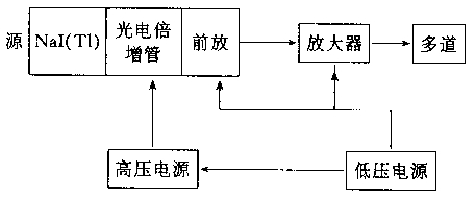
\includegraphics[width=0.6\textwidth]{fig/fig3.pdf}
	\caption{闪烁谱仪框图}\label{fig3}
\end{figure}

\subsection{谱仪组件性能一般介绍}
\begin{enumerate}
	\item 闪烁体:闪烁体时用来把射线能量转变为光能的。闪烁体分无机闪烁和有机闪烁体两大类。实际运用中依据不同的探测对象和要求选择不同的闪烁体。本实验中采用含铊(TI)的NaI晶体做$\gamma$射线的探测器。
	\item 光电倍增管:光电倍增管的结构如图所示。
	      它由光阴极K、收集电子的阳极A与在阳极与光阴极之间十个左右能发射二次电子的次阴极(又称倍增极、打拿极或者联极)构成,相邻的两个电极之间的电位差一般在100V左右。当闪烁体发出的光子达到光阴极时,它打出的光电子被加速聚焦到第一倍增极$D_1$上,平均每个光电子在$D_1$上打出了3$\sim$6个次级电子,增殖的电子又为$D_1$和$D_2$之间的电场加速,打到第二个倍增极$D_2$上,平均每个电子又打出3$\sim$5个次级电子,$\dots$这样经过n级倍增后,在阳极上就收集到大量的电子,在负载上形成一个电压脉冲。
	      \begin{figure}[!h]
		      \centering
		      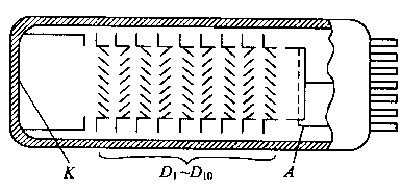
\includegraphics[width=0.5\textwidth]{fig/fig4.pdf}
		      \caption{百叶窗式非聚焦型光电倍增管}\label{fig4}
	      \end{figure}

	\item 能量分辨率:由于形成阳极电流脉冲之前的各种过程的统计性质,对应于某一定能量的粒子,光电倍增管的输出脉冲的幅度的大小仍有起伏,通常把脉冲计数率随脉冲幅度分布的半宽度$\Delta U_{1/2}$与计数率最大值对应的脉冲幅度$U_0$之比定义为能量分辨$\varepsilon$。
	      \begin{figure}[!h]
		      \centering
		      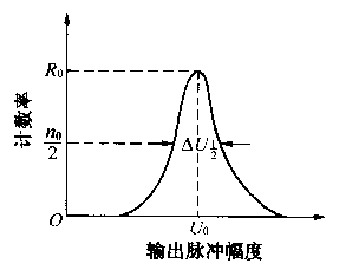
\includegraphics[width=0.5\textwidth]{fig/fig5.pdf}
		      \caption{输出脉冲幅度涨落所带来的对能量分辨本领的限制}\label{fig5}
	      \end{figure}

	      由于粒子能量与脉冲幅度成正比,所以能量分辨率
	      \begin{equation}
		      \varepsilon = \frac{\Delta U_{1/2}}{U_0} = \frac{\Delta E}{E}\label{eq13}
	      \end{equation}
	      影响能量分辨率的主要因素有:
	      \begin{enumerate}
		      \item 同一能量的粒子在闪烁体中产生的光子数目不同。这是由于
		            \begin{enumerate}
			            \item 闪烁体发光过程的统计涨落;
			            \item 闪烁体的非均性使不同点的发光效率不同;
			            \item 入射粒子穿过晶体的角度、位置不同所带来的在晶体内损失能量的不同。
		            \end{enumerate}
		      \item 粒子的入射位置不同,闪烁体所发出的光能到达光阴极的收集效率也不同。
		      \item 光阴极表面的不均匀性,阴极的不同位置发射光电子的效率不同。
		      \item 光阴极发射光电子数和光电倍增管的倍增系数的统计涨落。
		      \item 光电倍增管的本底脉冲噪声将叠加在入射粒子的脉冲信号上使之发生涨落。
	      \end{enumerate}
	      NaI(Tl)晶体对 的0.662MeV的 射线能量分辨率为6%$\sim$8%。
\end{enumerate}

\subsection{闪烁谱仪对$^{137}$Cs单能$\gamma$射线的响应}
$^{137}$Cs只放出单一能量的$\gamma$射线($E_{\gamma}$=0.662MeV),此$\gamma$射线能量小于正、负电子对的产生阈1.02MeV,所以Cs的$\gamma$射线于NaI(Tl)晶体的相互作用只有光电效应和康普顿散射两个过程,图(\ref{fig6})给出了用NaI(Tl)晶体$\gamma$谱仪所测得的$^{137}$Cs的$\gamma$能谱,其中1号峰相应于光电峰,1号峰左面的平台相应于康普顿电子的贡献。如果康普顿散射产生的散射光子$h\nu^{'}$未逸出晶体,仍然为NaI(Tl)晶体所吸收,也即通过光电效应把散射光子的能量$h\nu^{'}$转换成光电子能量,而这个光电子也将对输出脉冲作贡献。由于上述整个过程是在很短的时间内完成的,这个时间比探测器形成的一个脉冲所需的时间短得很多,所以先产生的康普顿电子和后产生的光电子,二者对输出脉冲的贡献是叠加在一起形成一个脉冲,这个脉冲幅度所对应的能量,是这两个电子的能量值和,即$E_e + h\nu^{'} = h\nu$。即等于入射$\gamma$射线的能量。所以这一过程所形成的脉冲将叠加在光电峰1之上使之增高。为了确切起见,1号峰又称为全能峰。
\begin{figure}[!h]
	\centering
	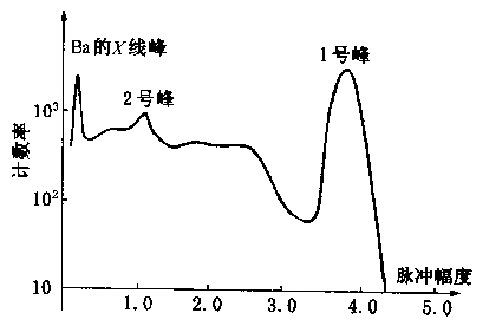
\includegraphics[width=0.6\textwidth]{fig/fig6.pdf}
	\caption{$^{137}$Cs的$\gamma$能谱}\label{fig6}
\end{figure}

上图的康普顿电子平台上还出现一个2号峰,它是由于入射$\gamma$射线穿过NaI晶体,达到光电倍增管上发生180$^{\circ}$的康普顿散射,反散射的光子返回晶体,与晶体发生光电效应所形成的。返回散射光子能量$h\nu^{'} = E_{\gamma} - E_{c(max)} = $0.184MeV,所以2号峰称为反散射峰。当然$\gamma$射线在源衬底、源容器材料上的反散射也会对反散射峰有贡献。

图中能量最小的那个峰是应为$^{137}$Cs的$\beta$衰变子体$^{137}$Bs在退激时,可能不发生$\gamma$射线,而是通过内转过程,把Ba的K电子打出,这一过程将导致发生Ba的K系X射线,所以这个峰对应于Ba的K系射线的能量(32keV左右)。

$^{137}$Cs的$\gamma$谱是比较典型的,常用$^{137}$Cs作为标准源,一方面用来检验$\gamma$谱仪的能量分辨率,另一方面作为$\gamma$射线能量测量的相对标准。

\subsection{闪烁谱仪的能量线性关系}
利用闪烁谱仪做$\gamma$射线能量测定时,最基本的要求是在入射$\gamma$射线的能量和它产生的脉冲幅度(指全能峰的位置)之间有确定的关系;对于理想的闪烁谱仪,脉冲幅度与能量之间应是线性关系;对于实际NaI(Tl)闪烁谱仪在较宽的能量范围内(100keV到1300keV)是近似线性的。这是利用该谱仪进行射线能量分析与判断未知放射性核素的重要依据。通常,在实验上利用系列$\gamma$标准源,测量相应全能量峰处的脉冲幅度,建立$\gamma$射线能量及其对应峰位的关系曲线,这条曲线即能量刻度曲线。典型的能量刻度曲线为不通过原点的一条直线,即
\begin{equation}
E(x_p) = Gx_p + E_0\label{eq14}
\end{equation}
式中$x_p$为全能峰位(峰道址);$E_0$为直线截距;$G$为增益(即单位脉冲幅度对应的能量)。能量刻度曲线可以选用标准源$^{137}$Cs(0.662MeV)和$^{60}$Co(1.17MeV,1.33MeV)来作,如图(\ref{fig7})所示。实验中欲得到较理想的线性,还要注意放大器和多道分析器甄别阈的线性,进行必要的检测与调整。此外,实验条件变化时应重新进行刻度。
\begin{figure}[!h]
	\centering
	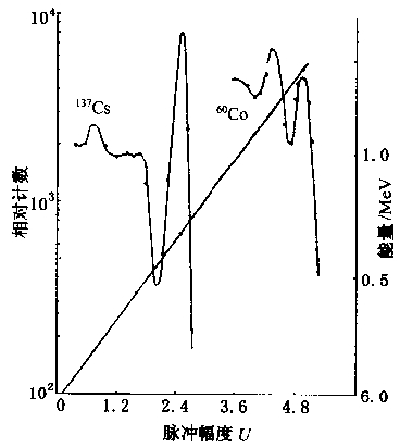
\includegraphics[width=0.5\textwidth]{fig/fig7.pdf}
	\caption{利用$^{60}$Co和$^{137}$Cs测定谱仪的能量刻度曲线}\label{fig7}
\end{figure}

\subsection{探测效率}
设$\gamma$源的发射强度为$S$,$\gamma$谱仪的探测效率为$\eta$,可以用下式表示:
\begin{equation}
\eta = \frac{n}{S}\label{eq15}
\end{equation}
(\ref{eq15})式中的$S$为$\gamma$射线发射强度,$n$为全能峰的总计数率,用这种方法定义的探测效率称作源峰探测效率,$n$可以用下式求得:
\begin{equation}
n = \frac{N}{t}\label{eq16}
\end{equation}
式中$N$为全能峰的净计数,$t$为计数时间。

全能峰的净计数$N$可采用全能峰面积法来计算(TPA法)具体步骤如下:
\begin{enumerate}
\item 选定所求的全能峰,在全能峰选定左,右两个边界道址$l$,$r$一般选在峰两侧的峰谷处。
\item 求得峰内各道计数的总和
\begin{equation*}
T = \sum\limits_{i=l}^rI_i
\end{equation*}
\item 计算本底计数
\begin{equation*}
B = \frac12(I_l+I_r)\cdot(r-l+1)
\end{equation*}
\item 计算净计数$N=T-B$及统计误差
\begin{equation*}
\sigma_N^2 = T + \frac12(r-l+1)\cdot B
\end{equation*}
\end{enumerate}

\subsection{辐射强度测量}
在相同条件下,分别测得标准源的全能峰面积$N_O$和待测样的全能峰面积$N_X$,设标准源的强度为$S_O$,待测样的强度为$S_X$,则有
\begin{equation}
S_X = \frac{N_X}{N_O}\cdot S_O\label{eq17}
\end{equation}

\section{实验内容}
\begin{enumerate}
\item 检查实验装置,打开电源,进入多道分析工作状态;
\item 选择合适的高压和放大倍数,使测得的$^{60}$Co标准源的两个全能峰道址在700到800之间;
\item 测量$^{60}$Co和$^{137}$Cs标准源的$\gamma$能谱,并根据测量结果对$\gamma$谱仪进行能量刻度,即求出(\ref{eq14})式中的常数$G$和$E_0$;
\item 测量$^{137}$Cs标准源的$\gamma$能谱,根据测得的能谱,计算$\gamma$谱仪的能量分辨率$\varepsilon$和探测效率$\eta$(已知标准源的发射强度$S_O = 75.3\times 10^3$/秒);
\item 测量待测$^{137}$Cs源的强度$S_X$;
\item 测量结束,先把高压降至0,再关机。
\end{enumerate}

\section{实验数据}
\subsection{数据}
\subsubsection{测量$\gamma$谱仪的能量分辨率$\varepsilon$及探测效率$\eta$}
计数时间:100秒;所用标准源$^{137}$Cs。

编号:26;源强$S_O = 66.6\times 10^3\text{Bq}$。

全能峰道址$x_0 = 312$,计数$n_0 = 517$;

半高宽左道址$x^{'} = 290$,右道址$x^{''} = 331$;

全能峰左边界道址$x_l = 254$,右道址$x_r = 352$;

全能峰净计数$N = 22787$。%,净面积$A = 20451$。

\subsubsection{测量$^{60}$Co标准源的$\gamma$能谱}
编号:12;源强$S_O = 79.1\times 10^3\text{Bq}$。

左全能峰道址$x_1 = 557$,右全能峰道址$x_2 = 631$;

左峰左边界道址$x_l = 524$,左峰右边界$x_r = 601$;

左峰净计数$N_O = 4031$。%,净面积$A = 1184$。

\subsubsection{测量$^{60}$Co待测源的$\gamma$能谱}
编号:11。%源强$S_X = 64.8\times 10^3\text{Bq}$。

左全能峰道址$x_1 = 553$,右全能峰道址$x_2 = 629$;

左峰左边界道址$x_l = 518$,左峰右边界$x_r = 590$;

左峰净计数$N_X = 3348$。

\subsection{计算}
\subsubsection{能量分辨率$\varepsilon$}
由(\ref{eq13})式可以推出$\gamma$谱仪的能量分辨率$\varepsilon$的计算公式,代入数据如下:
\begin{equation}
\varepsilon = \frac{\Delta U_{1/2}}{U_0} = \frac{\Delta x}{x_0} = \frac{331 - 290}{312}\times 100\% \doteq 13.14\%\label{varepsilon}
\end{equation}
\subsubsection{探测效率$\eta$}
由(\ref{eq15})、(\ref{eq16})式可计算探测效率$\eta$如下:
\begin{equation}
\eta = \frac{N}{S_Ot} = \frac{22787}{66.6\times 10^3\text{Bq} \times 100\text{s}}\times 100\% \doteq 0.34\%\label{eta}
\end{equation}
\subsubsection{$\gamma$辐射强度测量}
由(\ref{eq17})式可知待测源的辐射强度为:
\begin{equation}
S_{X\text{测量}} = \frac{N_X}{N_O}\cdot S_O = \frac{3348}{4031}\times 79.1\times 10^3 \doteq 65.7\times 10^3\text{Bq}\label{S_X}
\end{equation}
而实验手册中该编号的辐射源的辐射强度为:$S_{X\text{真实}} = 64.8\times 10^3\text{Bq}$,因此误差为:
\begin{equation}
\text{Error\%} = \frac{S_{X\text{测量}} - S_{X\text{真实}}}{S_{X\text{真实}}}\times 100\% \doteq 1.39\%\label{error}
\end{equation}
较小,说明该实验方法测量未知源的辐射强度较为准确。

\section{误差分析}
实验中主要的误差来源在于确定道址数时小范围内有多个符合条件的道址取值,有时峰较为不明显,导致读数困难并且因人而异带有较大的主观性。改进的方法是延长测量时间增加取样点数,使测得的图线更加平滑,峰和边界更加明显,道址的选取更加准确。

\section{思考题}

\subsection{$\gamma$射线与物质有哪三种主要作用,各有什么特点?}
$\gamma$射线与物质的相互作用主要是光电效应、康普顿散射和正负电子对产生三种过程。
\begin{enumerate}
\item 光电效应:入射$\gamma$光子把能量全部转移给原子中的束缚电子,将其打出形成光电子,光电子动能近似等于入射$\gamma$光子的能量。作用结束后光子消失,只剩下具有一定动能的自由电子。
\item 康普顿散射:入射$\gamma$光子与核外电子发生非弹性散射,康普顿电子能量在0至$E_{e(max)}$之间变化,其中$E_{e(max)}$如(2)式所示。作用结束后,光子能量减小,电子获得一定动能。
\item 正负电子对产生:入射$\gamma$射线能量超过2$m_ec^2$时,$\gamma$光子受原子核或电子的库仑场的作用可激发正负电子对。入射$\gamma$射线能量越大,产生正负电子对的几率也越大。在物质中正电子的寿命很短,当它在物质中耗尽自己的动能,便同物质原子中的轨道电子发生湮灭反应而变成一对能量各为$m_ec^2$的$\gamma$光子。
\end{enumerate}

\subsection{何为全能峰?全能峰的计数主要来自于哪些作用的贡献?}
$\gamma$光谱中由光电效应形成的光电峰能量与入射$\gamma$射线能量几乎相等,称为全能峰。其计数主要来源于光电效应形成的光电子,其能量为$h\nu$。此外,多次康普顿散射的累计效应和两个湮没光子被全吸收时的电子对效应,对全能峰也有贡献。康普顿散射过程中被散射的光子在闪烁体中发生光电作用产生的光电子$h\nu^{'}$加上康普顿电子$E_e$,并且有$E_e + h\nu^{'} = h\nu$,二者加在一起的脉冲对全能峰产生贡献。

\subsection{当改变源$\gamma$与探头之间的距离时,探测效率$\eta$有无变化?为什么?}
有变化。源向外发射的$\gamma$射线近似为球面波,那么,探测到的强度应和源与探头的距离的二次方成反比。$\gamma$源与探头之间的距离改变时,$\gamma$源对探头所张的立体角必然发生变化,$\gamma$光子被探头吸收的几率必然发生变化,从而引起探测效率的改变。

因此可见源与探头之间的距离改变会使$\eta$改变,所以在实验中不能随意改变探头与源的距离。

\subsection{在对$\gamma$辐射进行能量测量时,样品的位置改变时对测量的结果有无影响?为什么?}
没有影响。$\gamma$辐射的能量只取决于所用核素的种类,与样品位置的改变没有关系。因为在进行能量测量时,我们只关心$\gamma$光子的能量。而样品位置的改变只对探测得到的计数率有影响。
因为一个光子的能量在测量中一次性传递给探测器,所以样品位置的改变只影响到测量光子的数目,没有影响到光子产生的峰的道址。最终的结果是测量曲线的计数尺度减小,不影响峰值的位置。

\nocite{jiaocai}
\bibliography{ref}
\end{document}